\section{Results}
\label{sec:results}

% WRITING PROMPTS (comments only; they do not print). About 2 pages. Report
% facts here; keep the interpretation for the Discussion.
%
% The tables are generated from paper/data/ by
%   ros2 run lawn_mower_planning analyze_results paper/data/ordering-pioneer3at-direction.csv --tables paper/tables
% and the figures by paper/scripts/make_figures.py (see paper/scripts/README.md).
% "Ours" in the tables is the full method: the decomposition direction chosen
% by energy, then the GA order. Report the split of the gain (direction alone,
% ordering alone) with it; see src/lawn_mower_planning/README.md.
% They show the Pioneer 3-AT placeholder until the faculty robot runs are in.
%
% 1. Energy (Table ordering-energy, Fig. energy-results a). Ours uses less
%    energy than Xie et al. on every lawn and every seed: -10.3 % on average
%    (-6.4 % on random_3 to -14.2 % on two_beds), p = 0.002 over the lawns,
%    r = -1.00. With the same decomposition the difference is -3.3 %.
% 2. Where the gain comes from (Fig. energy-results b). Direction alone
%    (Xie et al. on our direction vs. Xie et al.): -7.3 % on average; ordering
%    alone: -3.3 %. Both are negative on every lawn.
% 3. Example (Fig. example-plans, three_beds, seed 0): 10.39 -> 9.30 -> 8.92 kJ
%    and 154 -> 115 -> 112 turns. Describe what the reader sees: the turned
%    lanes and the shorter transitions.
% 4. Other metrics (Table ordering-metrics): turns -24.4 %, path length -1.0 %
%    (not significant), connection length, coverage -0.8 points (explain the
%    clearance band), overlap, energy per mowed area -9.6 %.
% 5. Search quality (Fig. convergence): on the four 7-cell lawns the GA finds
%    the exact optimum in all 40 runs, at a median of 350 to 650 evaluations;
%    the PSO in 36 of 40. So 20 000 evaluations are ample on these lawns.
% 6. Planning time: 5.7 s against 2.4 s. Is that a problem for a mower that
%    plans once per lawn? Say so in one sentence here or in the Discussion.

% Generated by `ros2 run lawn_mower_planning analyze_results`; do not edit by hand.
% Regenerate it from the experiment CSV after every run.
\begin{table*}[t]
\centering
\caption{Energy of the coverage plan (kJ, mean $\pm$ standard deviation over 10 seeds) on the shared test lawns, robot model \texttt{pioneer3at}. $\Delta$: relative difference of our GA to Xie et al.; $p$: two-sided Wilcoxon signed-rank test over the seeds, Holm-corrected over the lawns. The optimum is exact (brute force) and only computed for lawns of up to 8 cells.}
\label{tab:ordering-energy}
\small
\setlength{\tabcolsep}{4pt}
\begin{tabular}{l r r r r r r r r}
\toprule
Lawn & Cells & Ours (GA) & Ours (PSO) & Xie et al. & Xie search, L+T & Optimum & $\Delta$ (\%) & $p$ \\
\midrule
\texttt{two\_beds} & 7 & 6.21 $\pm$ 0.00 & 6.22 $\pm$ 0.01 & 6.50 $\pm$ 0.00 & 6.27 $\pm$ 0.00 & 6.21 & $-4.32$ & 0.020 \\
\texttt{backyard} & 7 & 9.96 $\pm$ 0.00 & 9.96 $\pm$ 0.00 & 10.12 $\pm$ 0.00 & 9.96 $\pm$ 0.00 & 9.96 & $-1.61$ & 0.020 \\
\texttt{l\_shape} & 7 & 11.08 $\pm$ 0.00 & 11.08 $\pm$ 0.00 & 11.37 $\pm$ 0.00 & 11.10 $\pm$ 0.00 & 11.08 & $-2.60$ & 0.020 \\
\texttt{three\_beds} & 10 & 10.73 $\pm$ 0.00 & 10.73 $\pm$ 0.01 & 10.92 $\pm$ 0.03 & 10.74 $\pm$ 0.01 & -- & $-1.80$ & 0.020 \\
\texttt{garden} & 10 & 16.94 $\pm$ 0.00 & 16.97 $\pm$ 0.02 & 17.52 $\pm$ 0.18 & 16.99 $\pm$ 0.04 & -- & $-3.32$ & 0.020 \\
\texttt{park\_trees} & 13 & 21.98 $\pm$ 0.02 & 22.01 $\pm$ 0.03 & 22.25 $\pm$ 0.08 & 22.04 $\pm$ 0.01 & -- & $-1.23$ & 0.020 \\
\texttt{sports\_edge} & 13 & 26.24 $\pm$ 0.03 & 26.33 $\pm$ 0.05 & 26.63 $\pm$ 0.08 & 26.36 $\pm$ 0.03 & -- & $-1.45$ & 0.020 \\
\texttt{random\_1} & 10 & 12.76 $\pm$ 0.00 & 12.79 $\pm$ 0.03 & 13.23 $\pm$ 0.00 & 12.84 $\pm$ 0.05 & -- & $-3.58$ & 0.020 \\
\texttt{random\_2} & 15 & 13.72 $\pm$ 0.01 & 13.82 $\pm$ 0.03 & 14.35 $\pm$ 0.05 & 13.91 $\pm$ 0.05 & -- & $-4.35$ & 0.020 \\
\texttt{random\_3} & 7 & 13.41 $\pm$ 0.00 & 13.41 $\pm$ 0.00 & 13.62 $\pm$ 0.05 & 13.51 $\pm$ 0.00 & 13.41 & $-1.58$ & 0.020 \\
\midrule
All lawns & & \multicolumn{5}{l}{test over the 10 lawn means, rank-biserial $r = -1.00$} & $-2.58$ & 0.002 \\
\bottomrule
\end{tabular}
\end{table*}

% Generated by `ros2 run lawn_mower_planning analyze_results`; do not edit by hand.
% Regenerate it from the experiment CSV after every run.
\begin{table}[t]
\centering
\caption{Our GA against Xie et al.\ and against the search of Xie et al.\ with a length-and-turns objective on the same transition table (L+T), over all lawns and seeds, robot model \texttt{pioneer3at}. Means over all runs; $\Delta$: mean over the lawns of the relative difference of our GA, paired by seed; $p$: two-sided Wilcoxon signed-rank test over the lawn means; $r$: rank-biserial effect size.}
\label{tab:ordering-metrics}
\small
\setlength{\tabcolsep}{4pt}
\resizebox{\linewidth}{!}{%
\begin{tabular}{l r r r r r r r r}
\toprule
 & & \multicolumn{4}{c}{vs.\ Xie et al.} & \multicolumn{3}{c}{vs.\ L+T} \\
\cmidrule(lr){3-6} \cmidrule(lr){7-9}
Metric & Ours & Xie & $\Delta$ (\%) & $p$ & $r$ & $\Delta$ (\%) & $p$ & $r$ \\
\midrule
Energy (kJ) & 14.30 & 14.65 & $-2.58$ & 0.002 & $-1.00$ & $-0.51$ & 0.004 & $-1.00$ \\
Path length (m) & 1250.6 & 1273.8 & $-2.11$ & 0.004 & $-0.96$ & $+0.37$ & 0.039 & $+0.78$ \\
Turns & 180 & 184 & $-1.81$ & 0.002 & $-1.00$ & $-0.42$ & 0.297 & $-0.50$ \\
Connection length (m) & 36.5 & 54.8 & $-32.11$ & 0.006 & $-0.93$ & $+18.83$ & 0.008 & $+0.96$ \\
Coverage (\%) & 94.6 & 95.1 & $-0.52$ & 0.002 & $-1.00$ & $+0.06$ & 0.203 & $+0.51$ \\
Planning time (s) & 5.1 & 4.4 & $+19.43$ & 0.002 & $+1.00$ & $-25.62$ & 0.002 & $-1.00$ \\
\bottomrule
\end{tabular}}
\end{table}


\begin{figure*}[t]
\centering
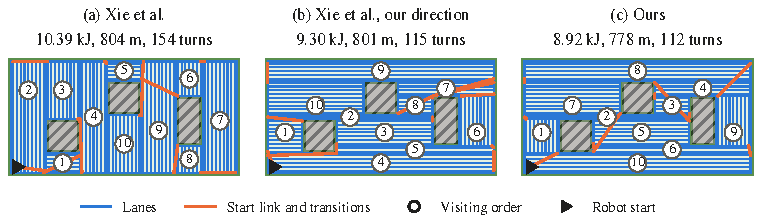
\includegraphics[width=\textwidth]{example-plans}
% DRAFT caption: rewrite in your own words.
\caption{Plans on the \texttt{three\_beds} lawn, seed 0. (a) Xie et al. (b) The ordering of Xie et al.\ on our decomposition direction. (c) Ours. Numbers give the visiting order of the cells.}
\label{fig:example-plans}
\end{figure*}

\begin{figure*}[t]
\centering
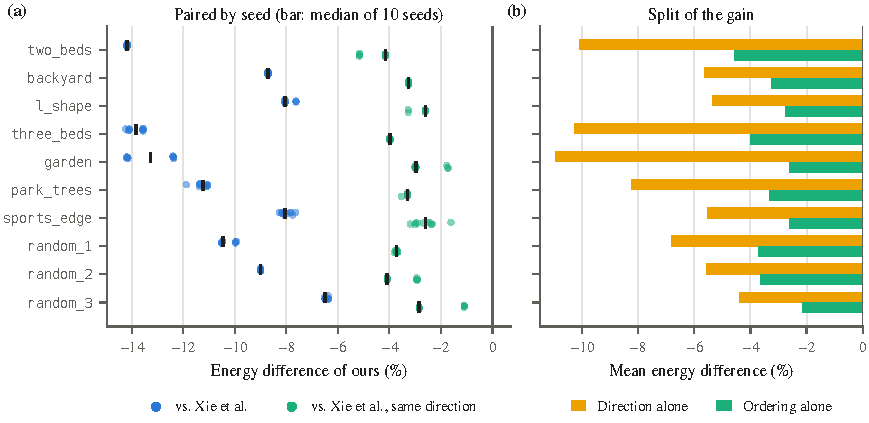
\includegraphics[width=\textwidth]{energy-results}
% DRAFT caption: rewrite in your own words.
\caption{Energy of our plans relative to the baseline, per lawn. (a) Paired difference for each of the 10 seeds, against Xie et al.\ and against Xie et al.\ on the same decomposition direction. (b) Mean difference due to the direction alone and to the ordering alone.}
\label{fig:energy-results}
\end{figure*}

\begin{figure*}[t]
\centering
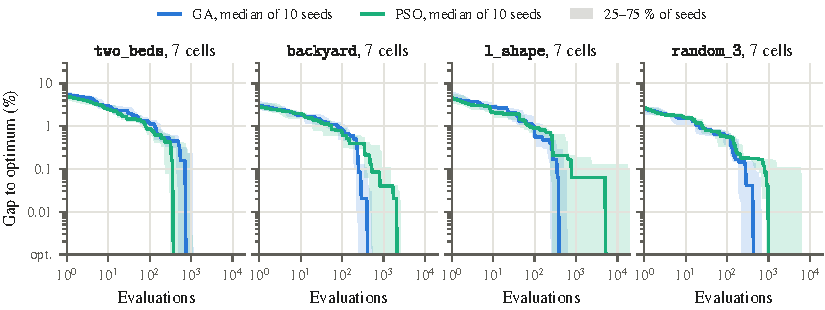
\includegraphics[width=\textwidth]{convergence}
% DRAFT caption: rewrite in your own words.
\caption{Gap of the best plan to the exact energy optimum during the search, on the four lawns of up to 8 cells (default direction). Lines: median of 10 seeds; bands: interquartile range.}
\label{fig:convergence}
\end{figure*}
